



Turning to support recovery problems in the Gaussian error model \eqref{eq:model-additive-Chapter3}, in the rest of this chapter
we will analyze the asymptotic performance limits in terms of the risk metrics for exact, exact-approximate, approximate-exact support recovery problems (i.e., \eqref{eq:risk-exact}, \eqref{eq:risk-exact-approx}, and \eqref{eq:risk-approx-exact}, respectively), as well as the probability of support recovery
\eqref{eq:risk-prob}.  We will also review the recent result for exact support recovery risk \eqref{eq:risk-approximate} by \cite{arias2017distribution}, to 
reveal a rather complete landscape of support recovery problems in high-dimensional Gaussian error models.


\begin{figure}
  \begin{center}
    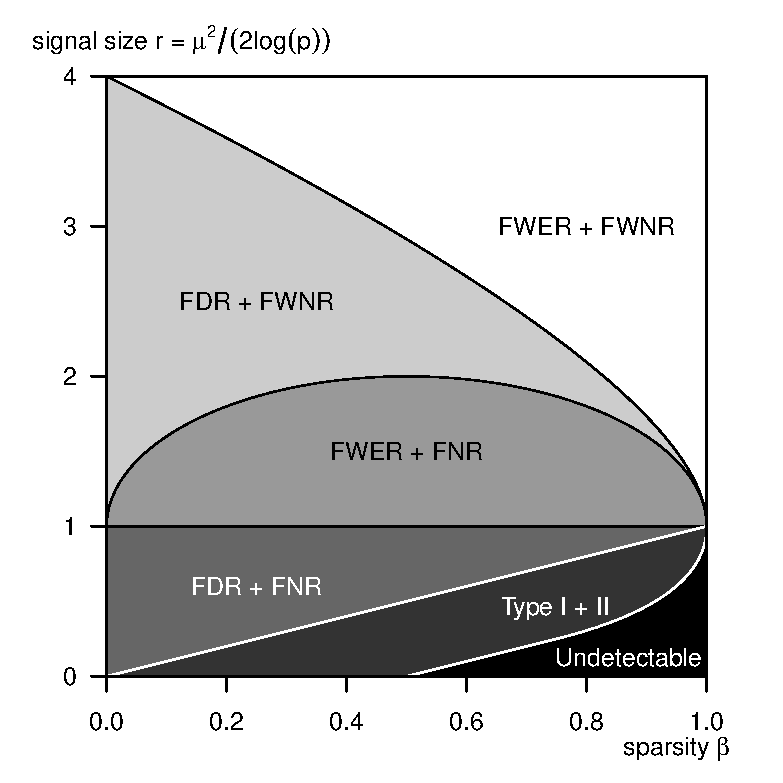
\includegraphics[width=0.7\textwidth]{./figures/theoretical_boundaries/phase_diagram_Gaussian_ALL_boundaries.eps}
  \end{center}
   \caption{The phase diagram of support recovery problems for the high-dimensional model \eqref{eq:model-additive-Chapter3}, illustrating the boundaries of the exact support recovery (FWER + FWNR; top curve; Theorem \ref{thm:Gaussian-error-exact-boundary}), the approximate-exact support recovery (FDR + FWNR; second curve from top; Theorem \ref{thm:Gaussian-error-approx-exact-boundary}), the exact-approximate support recovery (FWER + FNR; horizontal line $r=1$; Theorem \ref{thm:Gaussian-error-exact-approx-boundary}), and the approximate support recovery problems (FDR + FNR; tilted line $r=\beta$; Theorem \ref{thm:Gaussian-error-approx-boundary}). The signal detection problem (Type I + Type II errors of the global test; lower curve) was studied in Donoho and Jin (2004). In each region of the diagram and above, the annotated statistical risk can be made to vanish, as dimension $p$ diverges. Conversely, the risks has liminf at least one.}
   \label{fig:phase-Gaussian-errors}
\end{figure}

In the rest of this chapter, we restrict our attention to the class of thresholding procedures. Specifically, the lower bounds that we develop in 
Theorems \ref{thm:Gaussian-error-exact-boundary} through \ref{thm:Gaussian-error-approx-exact-boundary} below are only meant to apply to thresholding
 procedures.  Although it is intuitively appealing to consider only data-thresholding procedures in multiple testing problems, such procedures are not always optimal in more general settings. 
% Recently, \cite{arias2019detection} showed that thresholding procedures are in fact sub-optimal in the additive models \eqref{eq:model-additive} when errors have heavy (regularly-varying) tails. 
% Gao and Stoev [14] characterized the conditions under which thresholding procedures are optimal in the exact support recovery problem. 
% The optimality of data-thresholding procedures in terms of other statistical risks is an open problem that invites a dedicated investigation in a future study.
The optimality of thresholding procedures and the consequences of this restriction will be treated in Chapter \ref{chap:optimality}.


Figure \ref{fig:phase-Gaussian-errors} illustrates the rich landscape of phase transitions in support recovery for the various choices
of statistical risk for the family of thresholding estimators, established in the following sections.
We end this brief overview with a technical notion needed in order to state our main results.
We define a rate at which the nominal levels of FWER or FDR go to zero.
\begin{definition} \label{def:slowly-vanishing}
We say the nominal level of errors $\alpha = \alpha_p$ vanishes slowly, if
\begin{equation} \label{eq:slowly-vanishing-error}
    \alpha\to 0,\quad \text{and} \quad \alpha p^\delta\to\infty \text{  for any } \delta>0.
\end{equation}
\end{definition}
As an example, the sequence of nominal levels $\alpha_p = 1/\log{(p)}$ is slowly vanishing, while the sequence $\alpha_p = 1/\sqrt{p}$ is not.





\section{The exact support recovery problem}
\label{subsec:exact-support-recovery-Gaussian}

Our study of the exact support recovery risk \eqref{eq:risk-exact} begins with a brief review of existing results for the Hamming loss \eqref{eq:Hamming-loss}.
Indeed, as discussions in Section \ref{sec:asymptotics} suggest, the latter can be informative of the exact support recovery problems for models with independent components.

Inspired by the phase transition results for the signal detection problem, \cite{ji2012ups}, \citet{genovese2012comparison}, and \cite{jin2014optimality} derived interesting sharp results on support recovery problems in linear models under the Hamming loss $H(\widehat S, S)$.
Specifically, these papers establish minimax-type phase transition results in their respective settings. 
Under the sparsity parametrization in \eqref{eq:signal-sparsity-additive} and assuming equal signal sizes of ${(2r\log{p})^{1/2}}$, Hamming losses were shown to diverge to $+\infty$ when $r$ falls below the threshold
\begin{equation} \label{eq:strong-classification-boundary-Gaussian}
    f_{\mathrm{E}}(\beta) = (1 + (1 - \beta)^{1/2})^2,
\end{equation}
for any method of support estimation.
Conversely, under orthogonal, or near-orthogonal random designs, if $r>f_{\mathrm{E}}(\beta)$, they showed that the methods they proposed achieve vanishing Hamming loss.

Very recently, \citet{butucea2018variable}\; studied both asymptotics and non-asymptotics of support recovery problems in the additive noise model \eqref{eq:model-additive-Chapter3} under the assumption of equal signal sizes, using the Hamming loss.
Again, the analysis of asymptotic optimality focused on a newly proposed procedure which is very specific to the Gaussian model.
It is not at all clear if the optimality properties are a consequence of its mysterious construction.

We now show that commonly used and computationally efficient procedures can also be asymptotically optimal in the exact support recovery problem.

\begin{theorem} \label{thm:Gaussian-error-exact-boundary}
Consider the high-dimensional additive error model \eqref{eq:model-additive-Chapter3} under independent standard Gaussian errors, with signal sparsity and size as described in \eqref{eq:signal-sparsity-additive} and \eqref{eq:signal-size-additive}.
The function \eqref{eq:strong-classification-boundary-Gaussian} characterizes the phase transition of the exact support recovery problem.
Namely, the following two results hold.\\

{\rm (i)} If $\underline{r} > f_{\mathrm{E}}(\beta)$, then Bonferroni's, Sid\'ak's, Holm's, and Hochberg's procedures with slowly vanishing  nominal FWER levels 
(as defined in Definition \ref{def:slowly-vanishing}) all achieve asymptotically exact support recovery in the sense of \eqref{eq:support-recovery-success}. \\

{\rm (ii)} Conversely, if $\overline{r} < f_{\mathrm{E}}(\beta)$, then for any thresholding procedure $\widehat{S}_p$, we have $\P[\widehat{S}_p=S_p]\to0$.
Therefore, in view of Lemma \ref{lemma:risk-exact-recovery-probability}, exact support recovery asymptotically fails for all thresholding procedures in the sense of \eqref{eq:support-recovery-failure}.
\end{theorem}

We illustrate this result with a $\beta$-$r$ phase diagram in Figure \ref{fig:phase-Gaussian-errors}.  Theorem \ref{thm:Gaussian-error-exact-boundary} is in 
fact a special case of the more general Theorem \ref{thm:sufficient}, below, which covers dependent as well as Gaussain and non-Gaussian errors.  We will study the {\em exact support recovery} problem in greater detail and generality in Chapter \ref{chap:exact-support-recovery}. 


\section{The approximate support recovery problem}
\label{subsec:approx-support-recovery-Gaussian}

\cite{arias2017distribution} studied the performance of the Benjamini-Hochberg procedure \citep{benjamini1995controlling} and a stripped-down version of the Cand\'es-Barber procedure \citep{barber2015controlling} in approximate support recovery problems when the components of the noise term $\epsilon$ in \eqref{eq:model-additive-Chapter3} have independent and symmetric distributions.
A phase transition phenomenon for the approximate support recovery risk \eqref{eq:risk-approximate} was established in the Gaussian additive error model, where the two aforementioned methods are both shown to be asymptotically optimal.

The analysis therein, however, assumed equal signal sizes for the alternatives.
We generalize the main results of \citet{arias2017distribution} to allow for unequal signal sizes. 
The key to establishing this generalization is a monotonicity property of the \ac{BH} procedure, presented in the following 
Section \ref{sec:BH-monotonicity}. Namely, the power of the \ac{BH} procedure in terms of FNR monotonically increases for stochastically 
larger alternatives. This fact will be formalized in Lemma \ref{lemma:monotonicity-BH-procedure}, and may be of independent interest.


\begin{theorem} \label{thm:Gaussian-error-approx-boundary}
In the context of Theorem \ref{thm:Gaussian-error-exact-boundary}, the function 
\begin{equation} \label{eq:approx-boundary-Gaussian}
    f_{\mathrm{A}}(\beta) = \beta
\end{equation}
characterizes the phase transition of approximate support recovery problem.  Specifically the following two results hold.\\

{\rm (i)} If $\underline{r} > f_{\mathrm{a}}(\beta)$, then the Benjamini-Hochberg procedure (defined in Section \ref{sec:statistical-procedures}) with slowly 
vanishing nominal FDR levels (as defined in Definition \ref{def:slowly-vanishing}) achieves asymptotically approximate support recovery in the sense of \eqref{eq:support-recovery-success}.\\ 

{\rm (ii)}
Conversely, if $\overline{r} < f_{\mathrm{a}}(\beta)$, then approximate support recovery asymptotically fails in the sense of \eqref{eq:support-recovery-failure} for all thresholding procedures.
\end{theorem}


\begin{proof}[Necessary condition in Theorem \ref{thm:Gaussian-error-approx-boundary}]
We first show part {\rm (ii)}.  That is, when $\overline{r} < \beta$, no thresholding procedure is able to achieve approximate support recovery.
The arguments are similar to that in Theorem 1 of \cite{arias2017distribution}, although we allow for unequal signal sizes. 

Denote the distributions of $\mathrm{N}(0,1)$, $\mathrm{N}(\underline{\Delta}, 1)$, and $\mathrm{N}((\overline{\Delta}, 1)$ as $F_0$, $F_{\underline{a}}$, and $F_{\overline{a}}$ respectively.

% We first show the necessary condition, i.e., when $\overline{r}<\beta$, approximate support recovery cannot be achieved with any thresholding procedure.
% In particular, we show that the liminf of the sum of FDP and NDP is at least 1.

Recall that thresholding procedures are of the form
$$
\widehat{S}_p = \left\{i\,|\,x(i) > t_p(x)\right\}.
$$
Denote $\widehat{S} := \left\{i\,|\,x(i) > t_p(x)\right\}$, and $\widehat{S}(u) := \left\{i\,|\,x(i) > u\right\}$.
For any threshold $u\ge t_p$ we must have $\widehat{S}(u)\subseteq\widehat{S}$, and hence
\begin{equation} \label{eq:approx-boundary-proof-FDP-Gaussian}
    \text{FDP} := \frac{|\widehat{S}\setminus{S}|}{|\widehat{S}|} \ge \frac{|\widehat{S}\setminus{S}|}{|\widehat{S}\cup{S}|} = \frac{|\widehat{S}\setminus{S}|}{|\widehat{S}\setminus{S}| + |S|} \ge
    \frac{|\widehat{S}(u)\setminus{S}|}{|\widehat{S}(u)\setminus{S}| + |S|}.
\end{equation}
On the other hand, for any threshold $u\le t_p$ we must have $\widehat{S}(u)\supseteq\widehat{S}$, and hence
\begin{equation} \label{eq:approx-boundary-proof-NDP-Gaussian}
    \text{NDP} := \frac{|{S}\setminus\widehat{S}|}{|{S}|} \ge 
    \frac{|{S}\setminus\widehat{S}(u)|}{|{S}|}.
\end{equation}
Since either $u\ge t_p$ or  $u\le t_p$ must take place, putting \eqref{eq:approx-boundary-proof-FDP-Gaussian} and \eqref{eq:approx-boundary-proof-NDP-Gaussian} together, we have
\begin{equation} \label{eq:approx-boundary-proof-converse-1-Gaussian}
    \text{FDP} + \text{NDP} 
    \ge \frac{|\widehat{S}(u)\setminus{S}|}{|\widehat{S}(u)\setminus{S}|+|{S}|} \wedge \frac{|{S}\setminus\widehat{S}(u)|}{|{S}|},
\end{equation}
for any $u$.
Therefore it suffices to show that for a suitable choice of $u$, the RHS of \eqref{eq:approx-boundary-proof-converse-1-Gaussian} converges to 1 in probability; the desired conclusion on FDR and FNR follows by the dominated convergence theorem.

Let $t^* = \sqrt{2q\log{p}}$ for some fixed $q$, we obtain an estimate of the tail probability by Mill's ratio \eqref{eq:Mills-ratio}, 
\begin{equation}
    \overline{F_0}(t^*) 
    \sim \frac{1}{t^*}\phi(t^*)
    = \frac{1}{2\sqrt{\pi q\log{p}}} p^{-q}, \label{eq:approx-boundary-proof-null-tail-prob-Gaussian}
\end{equation}
where $a_p\sim b_p$ is taken to mean $a_p/b_p\to 1$.
Observe that $|\widehat{S}(t^*)\setminus{S}|$ has distribution $\text{Binom}(p-s, \overline{F_0}(t^*))$ where $s=|S|$, denote $X = X_p := {|\widehat{S}(t^*)\setminus{S}|}/{|S|}$, and we have 
$$
\mu := \E\left[X\right] = \frac{(p-s)\overline{F_0}(t^*)}{s},
\quad \text{and} \quad
\var\left(X\right) = \frac{(p-s)\overline{F_0}(t^*){F_0}(t^*)}{s^2} \le \mu/s.
$$
Therefore for any $M>0$, we have, by Chebyshev's inequality,
\begin{equation}
    \P\left[X < M\right] 
    \le \P\left[\left|X-\mu\right| > \mu - M\right]
    \le \frac{\mu/s}{(\mu-M)^2}
    = \frac{1/(\mu s)}{(1-M/\mu)^2}. \label{eq:approx-boundary-proof-converse-2-Gaussian}
\end{equation}
Now, from the expression of $\overline{F_0}(t^*)$ in \eqref{eq:approx-boundary-proof-null-tail-prob-Gaussian}, we obtain
$$
\mu = (p^\beta - 1)\overline{F_0}(t^*) \sim \frac{1}{2\sqrt{\pi q\log{p}}} p^{\beta-q}.
$$
Since $\overline{r}<\beta$, we can pick $q$ such that $\overline{r}<q<\beta$. 
In turn, we have $\mu \to\infty$, as $p\to\infty$.
Therefore the last expression in \eqref{eq:approx-boundary-proof-converse-2-Gaussian} converges to 0, and we conclude that $X\to\infty$ in probability, and hence
\begin{equation} \label{eq:approx-boundary-proof-converse-3-Gaussian}
\frac{|\widehat{S}(t^*)\setminus{S}|}{|\widehat{S}(t^*)\setminus{S}|+|{S}|} 
= \frac{X}{X+1} \to 1 \quad \text{in probability}.
\end{equation}

On the other hand, we show that with the same choice of $u = t^*$, we have,
\begin{equation} \label{eq:approx-boundary-proof-converse-4-Gaussian}
    \frac{|{S}\setminus\widehat{S}(t^*)|}{|{S}|}\to 1 \quad \text{in probability}.
\end{equation}
By the stochastic monotonicity of Gaussian location family \eqref{eq:stochastic-monotonicity-Gaussian}, we have the following lower bound for the probability of missed detection for each signal $\mu(i)$, $i\in S$, 
\begin{equation} \label{eq:approx-boundary-proof-converse-5-Gaussian}
    \P[\mathrm{N}(\mu(i), 1) \le t^*] \ge F_{\overline{a}}(t^*).
\end{equation}
Since $|{S}\setminus\widehat{S}(t^*)|$ can be written as the sum of $s$ independent Bernoulli random variables,
\begin{equation*}
    |{S}\setminus\widehat{S}(t^*)| = \sum_{i\in S} \mathbbm{1}_{(-\infty, t^*]}(x(i)),
\end{equation*}
using with \eqref{eq:approx-boundary-proof-converse-5-Gaussian}, we conclude that $|{S}\setminus\widehat{S}(t^*)| \stackrel{\mathrm{d}}{\ge} \text{Binom}(s, {F_{\overline{a}}}(t^*))$.
Finally, we know that ${F_{\overline{a}}}(t^*)$ converges to 1 by our choice of diverging $t^*$, and the necessary condition is shown.
\end{proof}


\begin{proof}[Sufficient condition in Theorem \ref{thm:Gaussian-error-approx-boundary}]
We now turn to the sufficient condition, i.e., part {\rm (i)}. That is, when $\underline{r} > \beta$, the Benjamini-Hochberg procedure with 
slowly vanishing FDR levels achieves asymptotic approximate support recovery.

The FDR vanishes by our choice of $\alpha$ and the FDR-controlling property of the BH procedure \citep{benjamini1995controlling}.
It only remains to show that FNR also vanishes.

To do so we compare the FNR under the alternative specified in Theorem \ref{thm:Gaussian-error-approx-boundary} to one with all of the signal sizes equal to $\underline{\Delta}$.
By Lemma \ref{lemma:monotonicity-BH-procedure}, it suffices to show that the FNR under the BH procedure in this setting vanishes.
Let $x(i)$ be vectors of independent observations with $p-s$ nulls having standard Gaussian distributions, and $s$ signals having $\mathrm{N}(\underline{\Delta}, 1)$ distributions.

Denote the null and the alternative distributions as $F_0$ and $F_{a}$ respectively.
Let $\widehat{G}$ denote the empirical survival function as in \eqref{eq:empirical-tail-distribution}.
Define the empirical survival functions for the null part and signal part
\begin{equation} \label{eq:empirical-survival-null-signal-Gaussian}
    \widehat{W}_\text{null}(t) = \frac{1}{p-s}\sum_{i\not\in S}\mathbbm{1}\{x(i) \ge t\},
    \quad
    \widehat{W}_\text{signal}(t) = \frac{1}{s}\sum_{i\in S}\mathbbm{1}\{x(i) \ge t\},
\end{equation}
where $s=|S|$, so that
$$
\widehat{G}(t) = \frac{p-s}{p}\widehat{W}_\text{null}(t) + \frac{s}{p}\widehat{W}_\text{signal}(t).
$$

We need the following result to describe the deviations of the empirical distributions.
\begin{lemma}[Theorem 1 of \citet{eicker1979asymptotic}] \label{lemma:empirical-process}
Let $Z_1,\ldots,Z_k$ be iid with continuous survival function $Q$.
Let $\widehat{Q}_k$ denote their empirical survival function and define 
$\xi_k = \sqrt{2\log{\log{(k)}}/k}$ for $k \ge 3$. 
Then
$$
\frac{1}{\xi_k}\sup_z\frac{|\widehat{Q}_k(z) - Q(z)|}{\sqrt{Q(z)(1 - Q(z))}} \to 1,
$$
in probability as $k \to \infty$.
In particular,
$$
\widehat{Q}_k(z) = Q(z) + O_\P\left(\xi_k\sqrt{Q(z)(1 - Q(z))}\right),
$$
uniformly in z.
\end{lemma}

Apply Lemma \ref{lemma:empirical-process} to the two summands in $\widehat{G}$, we obtain
$\widehat{G}(t) = G(t) + \widehat{R}(t)$,
where 
\begin{equation} \label{eq:empirical-process-mean-Gaussian}
    G(t) = \frac{p-s}{p}\overline{F_0}(t) + \frac{s}{p}\overline{F_a}(t),
\end{equation}
and 
\begin{equation} \label{eq:empirical-process-residual-Gaussian}
    \widehat{R}(t) = O_\P\left(\xi_p\sqrt{\overline{F_0}(t)F_0(t)} + \frac{s}{p}\xi_s\sqrt{\overline{F_a}(t)F_a(t)}\right),
\end{equation}
uniformly in $t$.

Recall (see proof of Lemma \ref{lemma:monotonicity-BH-procedure}) that the BH procedure is the thresholding procedure with threshold set at 
\begin{equation} \label{eq:approx-boundary-proof-tau-Gaussian}
    \tau = \inf\{t\,|\,\overline{F_0}(t)\le\alpha\widehat{G}(t)\}. 
    %= \min\{t\,|\,\overline{F_0}(t)=\alpha\widehat{G}(t)\}.
\end{equation}
The NDP may also be re-written as 
$$
\text{NDP} = \frac{|{S}\setminus\widehat{S}|}{|{S}|} = \frac{1}{s}\sum_{i\in S}\mathbbm{1}\{x(i) < \tau\} = 1 - \widehat{W}_\text{signal}(\tau),
$$
so that it suffices to show that 
\begin{equation} \label{eq:approx-boundary-proof-sufficient-1-Gaussian}
    \widehat{W}_\text{signal}(\tau)\to 1
\end{equation} in probability.
Applying Lemma \ref{lemma:empirical-process} to $\widehat{W}_\text{signal}$, we know that 
$$
\widehat{W}_\text{signal}(\tau) = \overline{F_a}(\tau) + O_\P\left(\xi_s\sqrt{\overline{F_a}(\tau)F_a(\tau)}\right) = \overline{F_a}(\tau) + o_\P(1).
$$
So it suffices to show that $F_a(\tau)\to 0$ in probability.
Now let $t^* = \sqrt{2q\log(p)}$ for some $q$ such that $\beta<q<\underline{r}$.
We have 
\begin{equation} \label{eq:approx-boundary-proof-sufficient-2-Gaussian}
    F_a(t^*) 
    = \Phi(t^* - \underline{\Delta}) 
    = \Phi(\sqrt{2(q - \underline{r})\log{p}}) \to 0. 
\end{equation}
Hence in order to show \eqref{eq:approx-boundary-proof-sufficient-1-Gaussian}, it suffices to show 
\begin{equation} \label{eq:approx-boundary-proof-sufficient-3-Gaussian}
    \P\left[\tau \le t^*\right] \to 1.
\end{equation}
By \eqref{eq:empirical-process-mean-Gaussian}, the mean of the empirical process $\widehat{G}$ evaluated at $t^*$ is
\begin{equation} \label{eq:approx-boundary-proof-sufficient-4-Gaussian}
    G(t^*) = \frac{p-s}{p}\overline{F_0}(t^*) + \frac{s}{p}\overline{F_a}(t^*).
\end{equation}
The first term, using Relation \eqref{eq:approx-boundary-proof-null-tail-prob-Gaussian}, is asymptotic to $p^{-q}L(p)$, where $L(p)$ is the logarithmic term in $p$.
The second term, since $\overline{F_a}(t^*)\to 1$ by Relation \eqref{eq:approx-boundary-proof-sufficient-2-Gaussian}, is asymptotic to $p^{-\beta}$.
Therefore, $G(t^*) \sim p^{-q}L(p) + p^{-\beta} \sim p^{-\beta}$, since 
$p^{\beta-q}L(p)\to0$ where $q>\beta$.

The fluctuation of the empirical process at $t^*$, by Relation \eqref{eq:empirical-process-residual-Gaussian}, is 
\begin{align*}
    \widehat{R}(t^*) 
    &= O_\P\left(\xi_p\sqrt{\overline{F_0}(t^*)F_0(t^*)} + \frac{s}{p}\xi_s\sqrt{\overline{F_a}(t^*)F_a(t^*)}\right)\\
    &= O_\P\left(\xi_p\sqrt{\overline{F_0}(t^*)}\right) + o_\P\left(p^{-\beta}\right).
\end{align*}
By \eqref{eq:approx-boundary-proof-null-tail-prob-Gaussian} and the expression for $\xi_p$, the first term is $O_\P\left(p^{-(q+1)/2}L(p)\right)$ where $L(p)$ is a poly-logarithmic term in $p$.
Since $\beta<\min\{q,1\}$, we have $\beta<(q+1)/2$, and hence $\widehat{R}(t^*) = o_\P(p^{-\beta})$.

Putting the mean and the fluctuation of $\widehat{G}(t^*)$ together, we obtain
$$
\widehat{G}(t^*) = G(t^*) + \widehat{R}(t^*) \sim_\P G(t^*) \sim p^{-\beta},
$$
and therefore, together with \eqref{eq:approx-boundary-proof-null-tail-prob-Gaussian}, we have
$$
\overline{F_0}(t^*)/\widehat{G}(t^*) = p^{\beta-q}L(p)(1+o_{\P}(1)),
$$
which is eventually smaller than the FDR level $\alpha$ by the assumption \eqref{eq:slowly-vanishing-error} and the fact that $\beta<q$.
That is, 
$$
\P\left[\overline{F}_0(t^*) / \widehat{G}(t^*) < \alpha\right] \to 1.
$$
By definition of $\tau$ (recall \eqref{eq:approx-boundary-proof-tau-Gaussian}), this implies that $\tau \le t^*$ with probability tending to 1, and \eqref{eq:approx-boundary-proof-sufficient-3-Gaussian} is shown.
The proof for the sufficient condition is complete.
\end{proof}


\section{Monotonicity of the Benjamini-Hochberg procedure}
\label{sec:BH-monotonicity}

As promised in the previous section, we make a connection between power of the \ac{BH} procedure and the stochastic ordering of distributions under the alternative.
This natural result seems new. 

\begin{lemma}[Monotonicity of the BH procedure] \label{lemma:monotonicity-BH-procedure}
Consider $p$ independent observations $x(i)$, $i\in\{1,\ldots,p\}$, where the $(p-s)$ coordinates in the null part have common distribution $F_0$, and the remaining $s$ signals have alternative distributions $F^{i}_j$, $i\in S$, respectively.
Compare the two alternatives $j\in\{1,2\}$, where the distributions in Alternative 2 are stochastically larger than those in Alternative 1, i.e.,
\begin{equation*}
    F^{i}_2(t) \le F^{i}_1(t), \quad \text{for all} \;\; t\in\R, \; \text{and for all} \;\; i\in S.
\end{equation*}
If the BH procedure is applied at the same nominal level of FDR, then the FNR of the \ac{BH} procedure under Alternative 2 is bounded above by the FNR under Alternative 1.
Further, the threshold of the \ac{BH} procedure under Alternative 2 is stochastically smaller than that under Alternative 1.
\end{lemma}

Loosely put, the power of the BH procedure is monotone increasing with respect to the stochastic ordering of the alternatives, yet (the distribution of) the \ac{BH} threshold is monotone decreasing in the distributions of the alternatives.

\begin{proof}[Lemma \ref{lemma:monotonicity-BH-procedure}]
We first re-express the BH procedure in a different form.
Recall that on observing $x(i)$, $i\in\{1,\ldots,p\}$, the BH procedure is the thresholding procedure with threshold set at $x_{[i^*]}$, where $i^* := \max\{i\,|\,\overline{F_0}(x_{[i]})\le \alpha i/p\}$, and $x_{[1]}\ge\ldots\ge x_{[p]}$ are the order statistics.

Let $\widehat{G}$ denote the left-continuous empirical survival function
\begin{equation} \label{eq:empirical-tail-distribution}
    \widehat{G}(t) = \frac{1}{p}\sum_{i=1}^p\mathbbm{1}\{x(i) \ge t\}.
\end{equation}
By the definition, we know that $\widehat{G}(x_{[i]}) = i/p$.
Therefore, by the definition of $i^*$, we have
\begin{equation*} 
    \overline{F_0}(x_{[i]}) > \alpha\widehat{G}(x_{[i]}) = \alpha i/p \quad \text{for all }i>i^*.
\end{equation*}
Since $\widehat{G}$ is constant on $(x_{[i^*+1]}, x_{[i^*]}]$, the fact that 
$\overline{F_0}(x_{[i^*]}) \le \alpha\widehat{G}(x_{[i^*]})$ and $\overline{F_0}(x_{[i^*+1]}) > \alpha\widehat{G}(x_{[i^*+1]})$ implies that $\alpha\widehat{G}$ and $\overline{F_0}$ must ``intersect'' on the interval by continuity of $F_0$.
We denote this ``intersection'' as
\begin{equation} \label{eq:approx-boundary-proof-tau}
    \tau = \inf\{t\,|\,\overline{F_0}(t)\le\alpha\widehat{G}(t)\}. 
    %= \min\{t\,|\,\overline{F_0}(t)=\alpha\widehat{G}(t)\}.
\end{equation}
Note that $\tau$ cannot be equal to $x_{[i^*+1]}$ since $\overline{F}_0$ is c\`adl\`ag.
Since there is no observation in $[\tau, x_{[i^*]})$, we can write the BH procedure as the thresholding procedure with threshold set at $\tau$.

Now, denote the observations under Alternatives 1 and 2 as $x_1(i)$ and $x_2(i)$.
Since $x_2(i)$ stochastically dominates $x_1(i)$ for all $i\in\{1,\ldots,p\}$, there exists a coupling $(\widetilde{x}_1, \widetilde{x}_2)$ of $x_1$ and $x_2$ such that 
% $\widetilde{x}_1(i) = \widetilde{x}_2(i)$ for $i\in S^c$, and 
$\widetilde{x}_1(i) \le \widetilde{x}_2(i)$ almost surely for all $i$.
We will replace $\widetilde{x}_1$ and $\widetilde{x}_2$ with $x_1$ and $x_2$ in what follows.
Since we will compare the FNR's, i.e., expectations with respect to the marginals of ${x}$'s in the last step, this replacement does not affect the conclusions.
To simplify notation, we still write $x_1$ and $x_2$ in place of $\widetilde{x}_1$ and $\widetilde{x}_2$.

Let $\widehat{G}_k$ be the left-continuous empirical survival function under Alternative $k$, i.e.,
\begin{equation} \label{eq:empirical-survival}
    \widehat{G}_k(t) = \frac{1}{p}\sum_{i=1}^p\mathbbm{1}\{x_k(i) \ge t\}, \quad k\in\{1,2\}.
\end{equation}
We define the BH thresholds $\tau_1$ and $\tau_2$ by replacing $\widehat{G}$ in \eqref{eq:approx-boundary-proof-tau} with $\widehat{G}_1$ and $\widehat{G}_2$, respectively.
Denote the set estimates of signal support $\widehat{S}_k = \{i\,|\,x_k(i)\ge\tau_k\}$ by the BH procedure.
We claim that 
\begin{equation} \label{eq:monotonicity-BH-procedure-thresholds}
    \tau_2 \le \tau_1 \quad \text{with probability } 1.
\end{equation}

Indeed, by definition of the empirical survival function \eqref{eq:empirical-survival} and the fact that $x_1(i) \le x_2(i)$ almost surely for all $i$,  we have $\widehat{G}_1(t) \le \widehat{G}_2(t)$ for all $t$.
Hence, $\overline{F_0}(t)\le\alpha\widehat{G}_1(t)$ implies $\overline{F_0}(t)\le\alpha\widehat{G}_2(t)$, and Relation \eqref{eq:monotonicity-BH-procedure-thresholds} follows from the definition of $\tau$ in \eqref{eq:approx-boundary-proof-tau}.
The claim of stochastic ordering of the \ac{BH} thresholds in Lemma \ref{lemma:monotonicity-BH-procedure} follows from \eqref{eq:monotonicity-BH-procedure-thresholds}.

Finally, when $\tau_2 \le \tau_1$, we have $\tau_2 \le \tau_1 \le x_1(i) \le x_2(i)$ with probability 1 for all $i\in\widehat{S}_1$.
Therefore, it follows that $\widehat{S}_1 \subseteq \widehat{S}_2$ and hence $|S\setminus\widehat{S}_2| \le |S\setminus\widehat{S}_1|$ almost surely. 
The first conclusion in Lemma \ref{lemma:monotonicity-BH-procedure} follows from the last inequality.
\end{proof}




\section{The exact-approximate support recovery problem}
\label{subsec:exact-approx-support-recovery-Gaussian}

We now derive two new asymptotic phase transition results for the \emph{asymmetric} statistical risks, \eqref{eq:risk-exact-approx} and \eqref{eq:risk-approx-exact}, in the Gaussian error models.
As discussed in Section \ref{sec:risks}, the exact-approximate support recovery risk is the natural criteria when considering the marginal power of discovery while controlling for family-wise error rates in applications such as GWAS.

Although there have been discussions of weighted sums of type I and type II errors in the literature (see, e.g., Genovese and Wasserman \citep{genovese2002operating} Section 6, where the authors sought to minimize $\textrm{FDR} + \lambda\textrm{FNR}$), asymptotic limits were not discussed.
We point out that the asymptotic limits for the unequally-weighted risks are no different from the equally-weighted risk, so long as $\lambda$ is bounded away from zero and infinity.
This is because $\textrm{FDR} + \lambda\textrm{FNR}$ vanishes if and only if both FDR and FNR vanish; conversely, non-vanishing FDR and FNR is equivalent to non-vanishing weighted sums.
Therefore, a different phase transition would only arise if we weight the type I and type II errors by combining family-wise error metrics with marginal error rates.

The next theorem describes the phase transition in the exact-approximate support recovery problem.

\begin{theorem} \label{thm:Gaussian-error-exact-approx-boundary}
In the context of Theorem \ref{thm:Gaussian-error-exact-boundary}, the function 
\begin{equation} \label{eq:exact-approx-boundary-Gaussian}
    f_{\mathrm{EA}}(\beta) = 1
\end{equation}
characterizes the phase transition of exact-approximate support recovery problem.  Namely, the following two results hold.\\

{\rm (i)} If $\underline{r} > f_{\mathrm{EA}}(\beta)$, then the procedures listed in Theorem \ref{thm:Gaussian-error-exact-boundary} with slowly vanishing nominal FWER levels (as defined in Definition \ref{def:slowly-vanishing}) achieve asymptotically exact-approximate support recovery in the sense of \eqref{eq:support-recovery-success}. \\

{\rm (ii)} Conversely, if $\overline{r} < f_{\mathrm{EA}}(\beta)$, then for any thresholding procedure $\widehat{S}$, the exact-approximate support recovery fails in the sense of \eqref{eq:support-recovery-failure}.
\end{theorem}

The phase transition boundary \eqref{eq:exact-approx-boundary-Gaussian} is visualized in Figure \ref{fig:phase-Gaussian-errors}. The proof of this result
uses ideas from the proof of Theorem \ref{thm:Gaussian-error-approx-boundary} and is substantially shorter.

\begin{proof}[Theorem \ref{thm:Gaussian-error-exact-approx-boundary}]
We first show the sufficient condition. 
Vanishing FWER is guaranteed by the properties of the procedures, and we only need to show that FNR also goes to zero. 
Similar to the proof of Theorem \ref{thm:Gaussian-error-approx-boundary}, it suffices to show that
\begin{equation} \label{eq:additive-error-exact-approx-boundary-proof-sufficient-1}
    \text{NDP} = 1 - \widehat{W}_\text{signal}(t_p) \to 0,
\end{equation}
where $t_p$ is the threshold of Bonferroni's procedure.

Since $\alpha$ vanishes slowly (see Definition \ref{eq:slowly-vanishing-error}), for any $\delta>0$, we have $p^{-\delta}=o(\alpha)$.
Therefore, we have $-\log\alpha\le\delta\log{p}$ for large $p$, and
\begin{equation*} 
    1 \le \limsup_{p\to\infty}\frac{2\log{p} - 2\log{\alpha}}{2\log{p}} \le 1+\delta,
\end{equation*}
for any $\delta>0$.
Therefore, by the expression for normal quantiles, we know that 
$$
t_p=F^\leftarrow(1-\alpha/p)\sim(2\log{p}-2\log{\alpha})^{1/2} \sim(2\log{p})^{1/2}.
$$

Since $\underline{r}>f_{\mathrm{EA}}(\beta)=1$, we can pick $q$ such that $1<q<\underline{r}$.
Let $t^* = \sqrt{2q\log{p}}$, we know that $t_p<t_p^*$ for large $p$.
Therefore for large $p$, we have
$$
\widehat{W}_\text{signal}(t_p) \ge \widehat{W}_\text{signal}(t^*) \ge \overline{F_a}(t^*) + o_\P(1),
$$
where $\overline{F_a}$ is the survival function of $\mathrm{N}(\sqrt{2\underline{r}\log{p}}, 1)$; the last inequality follows from the stochastic monotonicity of the Gaussian location family \eqref{eq:stochastic-monotonicity-Gaussian}, and Lemma \ref{lemma:empirical-process}.
Indeed, by our choice of $q<\underline{r}$, we obtain
$$
F_a(t^*) = \Phi\left(\sqrt{2(q-\underline{r})\log{p}}\right)\to0,
$$
and \eqref{eq:additive-error-exact-approx-boundary-proof-sufficient-1} is shown. 
This completes the proof of the sufficient condition.

The proof of the necessary condition follows similar structure as in the proof of Theorem \ref{thm:Gaussian-error-approx-boundary}, and uses the lower bound
\begin{equation} \label{eq:additive-error-exact-approx-boundary-proof-necessary-1}
    \mathrm{FWER}(\mathcal{R}) + \mathrm{FNR}(\mathcal{R}) \ge \P\left[\max_{i\in S^c}x(i)>u\right] \wedge \E\left[\frac{|S\setminus \widehat{S}(u)|}{|S|}\right],
\end{equation}
which holds for any arbitrary thresholding procedure $\mathcal{R}$ and arbitrary real $u\in\R$.

By the assumption that $\overline{r}<f_{\mathrm{EA}}(\beta)=1$, we can pick $q$ such that $\overline{r}<q<1$ and let $u = t^*=\sqrt{2q\log{p}}$ in \eqref{eq:additive-error-exact-approx-boundary-proof-necessary-1}.
By relative stability of iid Gaussian random variables \eqref{eq:relative-stability-Gaussian-maxima}, we have
\begin{equation} \label{eq:additive-error-exact-approx-boundary-proof-necessary-2}
    \P\left[\frac{\max_{i\in S^c} x(i)}{\sqrt{2\log{p}}} > \frac{t^*}{\sqrt{2\log{p}}}\right] \to 1.
\end{equation}
since the first fraction in \eqref{eq:additive-error-exact-approx-boundary-proof-necessary-2} converges to 1, while the second converges to $q<1$.
Therefore, the first term on the right-hand side of \eqref{eq:additive-error-exact-approx-boundary-proof-necessary-1} converges to 1.

On the other hand, by the stochastic monotonicity of Gaussian location family \eqref{eq:stochastic-monotonicity-Gaussian}, the probability of missed detection for each signal is lower bounded by $\P[Z+\mu(i) \le t^*] \ge F_{\overline{a}}(t^*)$, where $Z$ is a standard Gaussian r.v., and $F_{\overline{a}}$ is the cdf of $\mathrm{N}(\sqrt{2\overline{r}\log{p}}, 1)$.
Therefore, $|{S}\setminus\widehat{S}(t^*)| \stackrel{\mathrm{d}}{\ge} \text{Binom}(s, {F_{\overline{a}}}(t^*))$, and it suffices to show that ${F_{\overline{a}}}(t^*)$ converges to 1.
Indeed,
\begin{equation*}
    {F_{\overline{a}}}(t^*) = \Phi(\sqrt{2(q-\overline{r})\log{p}}) \to 1,
\end{equation*}
by our choice of $q>\overline{r}$.
Hence both quantities in the minimum on the right-hand side of \eqref{eq:additive-error-exact-approx-boundary-proof-necessary-1} converge to 1 in the limit, and the necessary condition is shown.
\end{proof}





\begin{remark}
The boundary \eqref{eq:exact-approx-boundary-Gaussian} was briefly suggested by \citet{arias2017distribution}.
Unfortunately, it was falsely claimed that the boundary characterized the phase transition of the \emph{exact} support recovery problem, and the alleged proof was left as an ``exercise to the reader''.
This exercise was completed in Chapter \ref{chap:exact-support-recovery}, where the correct boundary \eqref{eq:exact-boundary-chisquared} was identified. 

Theorem \ref{thm:Gaussian-error-exact-approx-boundary} here shows that the boundary \eqref{eq:exact-approx-boundary-Gaussian} \emph{does} exist, though for the slightly different \emph{exact-approximate} support recovery problem.
As we will see in Section \ref{sec:chisq-boundaries}, the boundary \eqref{eq:exact-approx-boundary-Gaussian} also applies to the exact-approximate support recovery problem in chi-square models \eqref{eq:model-chisq}.
\end{remark}

\section{The approximate-exact support recovery problem}
\label{subsec:aprox-exact-support-recovery-Gaussian}

The last phase transition is in terms of the approximate-exact support recovery risk
\eqref{eq:risk-approx-exact}.

\begin{theorem} \label{thm:Gaussian-error-approx-exact-boundary}
In the context of Theorem \ref{thm:Gaussian-error-exact-boundary}, the function 
\begin{equation} \label{eq:approx-exact-boundary-Gaussian}
    f_{\mathrm{AE}}(\beta) = \left(\sqrt{\beta} + \sqrt{1-\beta}\right)^2
\end{equation}
characterizes the phase transition of approximate-exact support recovery problem.  Namely, the following two results 
hold.\\

{\rm (i)} If $\underline{r} > f_{\mathrm{AE}}(\beta)$, then the Benjamini-Hochberg procedure with slowly vanishing nominal FDR levels (as defined in Definition \ref{def:slowly-vanishing}) achieves asymptotically approximate-exact support recovery in the sense of \eqref{eq:support-recovery-success}. \\

{\rm (ii)} Conversely, if $\overline{r} < f_{\mathrm{AE}}(\beta)$, then for any thresholding procedure $\widehat{S}$, the approximate-exact support recovery fails in the sense of \eqref{eq:support-recovery-failure}.
\end{theorem}

%Theorem \ref{thm:Gaussian-error-approx-exact-boundary} is proved in Section \ref{sec:proofs}.
The phase transition boundary \eqref{eq:approx-exact-boundary-Gaussian} is visualized in Figure \ref{fig:phase-Gaussian-errors}.

\begin{proof}[Theorem \ref{thm:Gaussian-error-approx-exact-boundary}]
We first show the sufficient condition (part {\rm (i)}).
Since FDR control is guaranteed by the BH procedure, we only need to show that the FWNR also vanishes, that is,
\begin{equation} \label{eq:approx-exact-boundary-proof-sufficient-1-Gaussian}
    \P\left[\min_{i\in S}x(i) \ge \tau\right] \to 1,
\end{equation}
where $\tau$ is the threshold for the BH procedure.

By the assumption that $\underline{r}>f_{\mathrm{AE}}(\beta)=(\sqrt{\beta}+\sqrt{1-\beta})^2$, we have $\sqrt{\underline{r}}-\sqrt{1-\beta}>\sqrt{\beta}$, so we can pick $q>0$, such that 
\begin{equation} \label{eq:approx-exact-boundary-proof-sufficient-2-Gaussian}
\sqrt{\underline{r}}-\sqrt{1-\beta}>\sqrt{q}>\sqrt{\beta}.
\end{equation}
We only need to show that with a specific choice of $t^*=\sqrt{2q\log{p}}$ where
\begin{equation} \label{eq:additive-error-approx-exact-boundary-proof-sufficient-1}
\sqrt{\underline{r}}-\sqrt{1-\beta}>\sqrt{q}>\sqrt{\beta},
\end{equation}
we have both
\begin{equation} \label{additive-error-eq:approx-exact-boundary-proof-sufficient-2}
\P\left[\tau\le t^*\right]\to 1,
\end{equation}
and 
\begin{equation} \label{eq:additive-error-approx-exact-boundary-proof-sufficient-3}
    \P\left[\min_{i\in S}x(i) \ge t^* \right] \to 1,
\end{equation}
so that 
\begin{equation*} 
    \P\left[\min_{i\in S}x(i) \ge \tau\right] \ge 
    % \P\left[\min_{i\in S}x(i) \ge t^* \ge \tau\right] \ge
    \P\left[\min_{i\in S}x(i) \ge t^*,\; t^* \ge \tau\right] \to 1.
\end{equation*}

Relation \eqref{additive-error-eq:approx-exact-boundary-proof-sufficient-2} follows in exactly the same way \eqref{eq:approx-boundary-proof-sufficient-3-Gaussian} did on page  \pageref{eq:approx-boundary-proof-sufficient-3-Gaussian}.

Dividing the left-hand-side in Relation \eqref{eq:additive-error-approx-exact-boundary-proof-sufficient-3} by $\sqrt{2\log{p}}$, we have,
\begin{align*}
    \frac{\min_{i\in S}x(i)}{\sqrt{2\log{p}}} 
    &= \frac{\min_{i\in S}\mu(i)+\epsilon(i)}{\sqrt{2\log{p}}} 
    \stackrel{\mathrm{d}}{\ge} \frac{\sqrt{2\underline{r}\log{p}} + \min_{i\in S}\epsilon(i)}{\sqrt{2\log{p}}} \\
    &\to -\sqrt{1-\beta} + \sqrt{\underline{r}},
\end{align*}
where the last convergence follows from the relative stability of iid Gaussians minima \eqref{eq:relative-stability-Gaussian-minima}. 
On the other hand, ${t^*}/{\sqrt{2\log{p}}}=\sqrt{q}<\sqrt{\underline{r}}-\sqrt{1-\beta}$ by our choice of ${q}$, and Relation \eqref{eq:additive-error-approx-exact-boundary-proof-sufficient-3} follows.


The necessary condition follows from the lower bound
\begin{equation} \label{eq:additive-error-approx-exact-boundary-proof-necessary-1}
    \mathrm{FDR}(\mathcal{R}) + \mathrm{FWNR}(\mathcal{R}) \ge \E\left[\frac{|\widehat{S}(u)\setminus S|}{|\widehat{S}(u)\setminus S| + |S|}\right] \wedge 
    \P\left[\min_{i\in S}x(i)<u\right],
\end{equation}
which holds for any thresholding procedure $\mathcal{R}$ and for arbitrary $u\in\R$.
In particular, we show that both terms in the minimum in \eqref{eq:additive-error-approx-exact-boundary-proof-necessary-1} converge to 1 when we set $u=t^*=\sqrt{2q\log{p}}$ where 
\begin{equation}
\sqrt{\overline{r}}-\sqrt{1-\beta}<\sqrt{q}<\sqrt{\beta}.
\end{equation}

On the one hand, we have,
$$
\frac{\min_{i\in S}x(i)}{\sqrt{2\log{p}}} 
\stackrel{\mathrm{d}}{\le} \frac{\min_{i\in S}\epsilon(i)+\sqrt{2\overline{r}\log{p}}}{\sqrt{2\log{p}}} 
\to \sqrt{\overline{r}}-\sqrt{1-\beta},
$$
by relative stability of iid Gaussians \eqref{eq:relative-stability-Gaussian-minima}. On the other hand, ${t^*}/{\sqrt{2\log{p}}}=\sqrt{q}>\sqrt{\underline{r}}-\sqrt{1-\beta}$ by our choice of ${q}$;
this shows that the second term on the right-hand side of \eqref{eq:additive-error-approx-exact-boundary-proof-necessary-1} converges to 1.

Observe that $|\widehat{S}(t^*)\setminus{S}|$ has distribution $\text{Binom}(p-s, \overline{\Phi}(t^*))$, and define $X = X_p := {|\widehat{S}(t^*)\setminus{S}|}/{|S|}$, we obtain,
% On the other hand, define $ = \E[|S\setminus\widehat{S}(t^*)|/|S|]$,
\begin{align*}
    \mu &:= \E[X] = (p^\beta-1)\overline{\Phi}(t^*) 
    \sim (p^\beta-1)\frac{\phi(t^*)}{t^*} \\
    &\sim \frac{1}{\sqrt{2\pi}}\left(2q\log{p}\right)^{-1/2}p^{\beta-q}\to\infty,
\end{align*}
where the divergence follows from our choice of $q<\beta$.
Using again Relations \eqref{eq:approx-boundary-proof-converse-2-Gaussian} and \eqref{eq:approx-boundary-proof-converse-3-Gaussian}, we conclude that the first term on the right-hand side of \eqref{eq:additive-error-approx-exact-boundary-proof-necessary-1} also converges to 1.
This completes the proof of the necessary condition.
\end{proof}


\section{Asymptotic power analysis: A discussion}
\label{subsec:power-analysis}

%We end this chapter with a general discussion on the effect of the signal sparsity on the interplay between 
%signal size and sparsity in the context of the detection and
% support recovery problems.  Specifically, different support recovery criteria are compared.
 
Theorems \ref{thm:Gaussian-error-exact-boundary} through \ref{thm:Gaussian-error-approx-exact-boundary} allow us to asymptotically quantify the required signals sizes in support recovery problems, as well as in the global hypothesis testing problem in the Gaussian additive error model \eqref{eq:model-additive-Chapter3}. 
Specifically, these results indicate that at all sparsity levels $\beta\in(0,1)$, the difficulties of the problems in terms of the required signal sizes have the following ordering
$$
f_{\mathrm{D}}(\beta) < f_{\mathrm{A}}(\beta) < f_{\mathrm{EA}}(\beta) < f_{\mathrm{AE}}(\beta) < f_{\mathrm{E}}(\beta),
$$
as previewed in Figure \ref{fig:phase-Gaussian-errors}.
The ordering aligns with our intuition that the required signal sizes must increase as we move from detection to support recovery problems.
Similarly, more stringent criteria for error control (e.g., FWER compared to FDR) require larger signals.
We can now also compare $f_{\mathrm{EA}}(\beta)$ and $f_{\mathrm{AE}}(\beta)$, whose ordering may not be clear from this line of reasoning.


\medskip

Our last comment is on the gap between FDR and FWER under sparsity assumptions. 
Although it is believed that FWER control is sometimes too stringent compared to, say, FDR control in support recovery problems, the fact that all five thresholds involve the same scaling indicates that the difficulties of the problems (signal detection, and the four support recovery problems) are comparable when signals are very sparse, i.e., when $\beta$ is close to 1.
This is illustrated with the next example.

\begin{example}[Power analysis for variable selection] \label{exmp:gap-when-signal-sparse}
For Gaussian errors (AGG with $\nu = 2$), when $\beta = 3/4$, the signal detection boundary \eqref{eq:detection-boundary-large-signals} says that signals will have to be at least of magnitude $\sqrt{(\log{p})/2}$, 
while approximate support recovery \eqref{eq:approx-boundary-Gaussian} requires signal sizes of at least $\sqrt{3(\log{p})/2}$, 
and exact support recovery \eqref{eq:strong-classification-boundary-Gaussian} calls for signal sizes of at least $\sqrt{9(\log{p})/2}$. 
The required signal sizes increases, but are within the same order of magnitude.

If $m$ independent copies $x_1,\ldots,x_m$ of the observations were made on the same set of $p$ locations, then by taking location-wise averages, $\overline{x}_{m}(j) = \frac{1}{m}\sum_{i=1}^{m} x_i(j)$,
we can reduce error standard deviation, and hence boost the signal-to-noise ratio, by a factor of $\sqrt{m}$.
By the simple calculations above, if $m$ samples are needed to detect (sparse) signals of a certain magnitude, then $3m$ samples will enable approximate support recovery with false discovery and non-discovery control, and in fact, $9m$ samples would enable exact support recovery with family-wise error rates control.
\end{example}

On the other hand, the gap between FDR and FWER is much larger when signals are dense.
For example, if the signals are only \emph{approximately} sparse, i.e., having a few components above \eqref{eq:strong-classification-boundary-Gaussian} but many smaller components above  \eqref{eq:approx-boundary-Gaussian}, then FDR-controlling procedures will discover substantially larger proportion of signals than FWER-controlling procedures.

Indeed, as $\beta\to0$, the required signal size for approximate support recovery \eqref{eq:approx-boundary-Gaussian} tends to 0, while the required signal size for exact support recovery \eqref{eq:strong-classification-boundary-Gaussian} tends to $4$ in the Gaussian error models.
While Example \ref{exmp:gap-when-signal-sparse} indicates that the exact support recovery is not much more stringent than approximate support recovery when signals are sparse, the gap between required signal sizes widens when signals are dense. 

